\documentclass[11pt, oneside]{article}\usepackage[]{graphicx}\usepackage[]{color}
%% maxwidth is the original width if it is less than linewidth
%% otherwise use linewidth (to make sure the graphics do not exceed the margin)
\makeatletter
\def\maxwidth{ %
  \ifdim\Gin@nat@width>\linewidth
    \linewidth
  \else
    \Gin@nat@width
  \fi
}
\makeatother

\definecolor{fgcolor}{rgb}{0.345, 0.345, 0.345}
\newcommand{\hlnum}[1]{\textcolor[rgb]{0.686,0.059,0.569}{#1}}%
\newcommand{\hlstr}[1]{\textcolor[rgb]{0.192,0.494,0.8}{#1}}%
\newcommand{\hlcom}[1]{\textcolor[rgb]{0.678,0.584,0.686}{\textit{#1}}}%
\newcommand{\hlopt}[1]{\textcolor[rgb]{0,0,0}{#1}}%
\newcommand{\hlstd}[1]{\textcolor[rgb]{0.345,0.345,0.345}{#1}}%
\newcommand{\hlkwa}[1]{\textcolor[rgb]{0.161,0.373,0.58}{\textbf{#1}}}%
\newcommand{\hlkwb}[1]{\textcolor[rgb]{0.69,0.353,0.396}{#1}}%
\newcommand{\hlkwc}[1]{\textcolor[rgb]{0.333,0.667,0.333}{#1}}%
\newcommand{\hlkwd}[1]{\textcolor[rgb]{0.737,0.353,0.396}{\textbf{#1}}}%
\let\hlipl\hlkwb

\usepackage{framed}
\makeatletter
\newenvironment{kframe}{%
 \def\at@end@of@kframe{}%
 \ifinner\ifhmode%
  \def\at@end@of@kframe{\end{minipage}}%
  \begin{minipage}{\columnwidth}%
 \fi\fi%
 \def\FrameCommand##1{\hskip\@totalleftmargin \hskip-\fboxsep
 \colorbox{shadecolor}{##1}\hskip-\fboxsep
     % There is no \\@totalrightmargin, so:
     \hskip-\linewidth \hskip-\@totalleftmargin \hskip\columnwidth}%
 \MakeFramed {\advance\hsize-\width
   \@totalleftmargin\z@ \linewidth\hsize
   \@setminipage}}%
 {\par\unskip\endMakeFramed%
 \at@end@of@kframe}
\makeatother

\definecolor{shadecolor}{rgb}{.97, .97, .97}
\definecolor{messagecolor}{rgb}{0, 0, 0}
\definecolor{warningcolor}{rgb}{1, 0, 1}
\definecolor{errorcolor}{rgb}{1, 0, 0}
\newenvironment{knitrout}{}{} % an empty environment to be redefined in TeX

\usepackage{alltt} 
\usepackage{amsmath}
\usepackage{amsthm}
\usepackage[margin=1in]{geometry} 
\usepackage{enumitem}
\usepackage{hhline}

\newenvironment{solution}
  {\begin{proof}[Solution]}
  {\end{proof}}
  
\usepackage{sectsty}
\sectionfont{\fontsize{12}{15}\selectfont}

\title{Directed Graphical Models}
\author{Skye Hersh \\ Modern Computational Statistics}
\IfFileExists{upquote.sty}{\usepackage{upquote}}{}
\begin{document} %%%%%%%%%%%%%%%%%%%%%%%%%%%%%%%%%%%%%%%%%%%%%%%%%%%%%%%%%%%%%%%%%%%
\maketitle

\section*{Bishop, Chapter 8}
\subsection*{8.3}
Consider three binary variables $a, b, c\ \epsilon\ \{0, 1\}$ having the joint distribution given in the table below. Show by direct evaluation that this distribution has the property that $a$ and $b$ are marginally dependent, so that $p(a, b) ≠ p(a)p(b)$, but that they become independent when conditioned on $c$, so that $p(a, b|c) = p(a|c)p(b|c)$ for both $c = 0$ and $c = 1$.

  \begin{table}[h!]
  \centering
  \begin{tabular}{ |c|c|c|c| }
  \hline
  $a$ & $b$ & $c$ & $p(a, b, c)$ \\
  \hline
  0 & 0 & 0 & .192 \\
  0 & 0 & 1 & .144 \\
  0 & 1 & 0 & .048 \\ 
  0 & 1 & 1 & .216 \\
  1 & 0 & 0 & .192 \\
  1 & 0 & 1 & .064 \\
  1 & 1 & 0 & .048 \\
  1 & 1 & 1 & .096 \\
  \hline
  \end{tabular}
  \end{table}

\begin{solution}\mbox{} \newline

We can decompose the discrete distribution $p(a, b)$ into four respective probabilities for the four combinations that the variables $a$ and $b$ can take on: that for when $(a=0, b=0)$; $(a=0, b=1)$; $(a=1, b=0)$; and when $(a=1, b=1)$. 

As $a$ and $b$ are Bernoulli random variables, we can begin by finding the marginal probabilities for either possible outcome for either variable by itself, summing over the rows in the table wherein such outcome's condition is met, e.g., $$ p(a=0) = \sum_b \sum_c p(a=0, b, c). $$

Thus, we find that 

  \begin{align}
  p(a=0) &= 0.192 + 0.144 + 0.048 + 0.216 \\
  &= 0.600.
  \end{align}

According to the same principle, we have

$$ p(a=1) = 0.400 $$
$$ p(b=0) = 0.592 $$
$$ p(b=1) = 0.408. $$

(Sensibly, $p(a=0) + p(a=1) = p(b=0) + p(b=1) = 1.$) The joint probability distribution $ p(a, b) $ comprises four discrete probabilities — one for each combination of the variables' binary outcomes — wherein, for example, $$ p(a=0, b=0) = \sum_c p(a=0, b=0, c). $$

From the table and the marginal probabilities worked out above, we have that

  \begin{table}[h!]
  \centering
  \begin{tabular}{ |c|c|c|c| }
  \hline
  $a$ & $b$ & $p(a, b)$ & $p(a)p(b)$ \\ 
  \hline
  0 & 0 & $0.192 + 0.144 = 0.336$ & $0.6 × 0.592 = 0.3552$ \\
  0 & 1 & $0.048 + 0.216 = 0.264$ & $0.6 × 0.408 = 0.2448$ \\
  1 & 0 & $0.192 + 0.064 = 0.256$ & $0.4 × 0.592 = 0.2368$ \\
  1 & 1 & $0.048 + 0.096 = 0.144$ & $0.4 × 0.408 = 0.1632$ \\
  \hline
  \end{tabular}
  \end{table}

Immediately, we see that in every case, $p(a, b) ≠ p(a)p(b),$ as $a$ and $b$ are marginally dependent. On the other hand, we find that they become independent when conditioned on $c$. We know that $$p(a|c) = \frac{p(a, c)}{p(c)},$$ $$p(b|c) = \frac{p(b, c)}{p(c)},$$ $$p(a, b|c) = \frac{p(a, b, c)}{p(c)}.$$ 

Noting that $p(c=0) = 0.48$ and $p(c=1) = 0.52$, we can compute the marginal, conditional probabilities accordingly:

  \begin{table}[h!]
  \centering
  \begin{tabular}{ |c|c|c|c|c|c|c| }
  \hline
  $a$ & $b$ & $c$ & $p(a|c)$ & $p(b|c)$ & $p(a, b|c)$ & $p(a|c)p(b|c)$ \\
  \hline
  \rule{0pt}{3ex} 0 & 0 & 0 & $\frac{0.240}{0.480}=0.500$ & $\frac{0.384}{0.480}=0.800$ & $\frac{.192}{0.480} = 0.400$ & $0.500\times0.800= 0.400$ \\
  \rule{0pt}{3ex} 0 & 0 & 1 & $\frac{0.360}{0.520}\approx0.692$ & $\frac{0.208}{0.520}=0.400$ & $\frac{.144}{0.520}\approx 0.277$ & $0.692\times0.400\approx0.277$ \\
  \rule{0pt}{3ex} 0 & 1 & 0 & $\frac{0.240}{0.480} = 0.500$ & $\frac{0.096}{0.480} = 0.200$ & $\frac{.048}{0.480} = 0.100$ & $0.500\times0.200=0.100$ \\
  \rule{0pt}{3ex} 0 & 1 & 1 & $\frac{0.360}{0.520} \approx 0.692$ & $\frac{0.312}{0.520} = 0.600$ & $\frac{.216}{0.520} \approx 0.415$ & $0.692\times0.600=0.415$ \\
  \rule{0pt}{3ex} 1 & 0 & 0 & $\frac{0.240}{0.480} = 0.500$ & $\frac{0.384}{0.480} = 0.800$ & $\frac{.192}{0.480} = 0.400$ & $0.500\times0.800=0.400$ \\
  \rule{0pt}{3ex} 1 & 0 & 1 & $\frac{0.160}{0.520} \approx 0.307$ & $\frac{0.208}{0.520} = 0.400$ & $\frac{.064}{0.520} \approx 0.123$ & $0.307\times0.400\approx0.123$ \\
  \rule{0pt}{3ex} 1 & 1 & 0 & $\frac{0.240}{0.480} = 0.500$ & $\frac{0.096}{0.480} = 0.200$ & $\frac{.048}{0.480} = 0.100$ & $0.500\times0.200=0.100$ \\
  \rule{0pt}{3ex} 1 & 1 & 1 & $\frac{0.160}{0.520} \approx 0.308$ & $\frac{0.312}{0.520} = 0.600$ & $\frac{.096}{0.520} \approx 0.185$ & $0.308\times0.600\approx0.185$ \\
  \hline
  \end{tabular}
  \end{table}
  
The latter two columns show the equivalence between $p(a, b|c)$ and $p(a)p(b)$.

\end{solution}

\subsection*{8.4}
Evaluate the distributions $p(a)$, $p(b|c)$, and $p(c|a)$ corresponding to the joint
distribution given in the original table. Hence show by direct evaluation that $p(a, b, c)$ =
$p(a)p(c|a)p(b|c)$. Draw the corresponding directed graph.

\begin{solution}\mbox{} \newline

We have the distributions for $p(a)$ and $p(b|c)$ above. The distribution $p(c|a) = \frac{p(a, c)}{p(a)}$ can be written accordingly:

\begin{table}[h]
\centering
\begin{tabular}{|c|c|c|}
\hline
$a$ & $c$ & $p(c|a)$ \\
\hline
0 & 0 & $\frac{0.240}{0.600} = 0.400$ \\
0 & 1 & $\frac{0.360}{0.600} = 0.600$ \\
1 & 0 & $\frac{0.240}{0.400} = 0.600$ \\
1 & 1 & $\frac{0.160}{0.400} = 0.400$ \\
\hline
\end{tabular}
\end{table}

From here, we can complete the following table, demonstrating the equivalency of $p(a)p(c|a)p(b|c)$ and $p(a)p(c|a)p(b|c)$.

\begin{table}[h]
\centering
\begin{tabular}{|c|c|c|c|c|}
\hline
$a$ & $b$ & $c$ & $p(a)p(c|a)p(b|c)$ & $p(a)p(c|a)p(b|c)$  \\
\hline
0 & 0 & 0 & $0.600\times0.400\times0.800=0.192$ & $0.192$  \\
0 & 0 & 1 & $0.600\times0.600\times0.400=0.144$ & $0.144$  \\
0 & 1 & 0 & $0.600\times0.400\times0.200=0.048$ & $0.048$  \\
0 & 1 & 1 & $0.600\times0.600\times0.600=0.216$ & $0.216$  \\
1 & 0 & 0 & $0.400\times0.600\times0.800=0.192$ & $0.192$  \\
1 & 0 & 1 & $0.400\times0.400\times0.400=0.064$ & $0.064$  \\
1 & 1 & 0 & $0.400\times0.600\times0.200=0.048$ & $0.048$  \\
1 & 1 & 1 & $0.400\times0.400\times0.600=0.096$ & $0.096$  \\
\hline
\end{tabular}
\end{table}

\end{solution}

\begin{knitrout}
\definecolor{shadecolor}{rgb}{0.969, 0.969, 0.969}\color{fgcolor}\begin{kframe}
\begin{alltt}
\hlkwd{suppressMessages}\hlstd{(}\hlkwd{library}\hlstd{(igraph))}
\hlstd{g} \hlkwb{<-} \hlkwd{graph_from_literal}\hlstd{(A}\hlopt{-+}\hlstd{C}\hlopt{-+}\hlstd{B)}
\hlkwd{plot.igraph}\hlstd{(g,} \hlkwc{edge.color} \hlstd{=} \hlstr{"black"}\hlstd{,} \hlkwc{vertex.color} \hlstd{=} \hlstr{"white"}\hlstd{,}
            \hlkwc{vertex.label} \hlstd{=} \hlkwd{c}\hlstd{(}\hlstr{"A"}\hlstd{,}\hlstr{"C"}\hlstd{,}\hlstr{"B"}\hlstd{),} \hlkwc{vertex.size} \hlstd{=} \hlnum{45}\hlstd{,} \hlkwc{vertex.label.cex} \hlstd{=} \hlnum{4}\hlstd{,}
            \hlkwc{vertex.label.color} \hlstd{=} \hlstr{"black"}\hlstd{,} \hlkwc{edge.width} \hlstd{=} \hlnum{1}\hlstd{,} \hlkwc{edge.arrow.size} \hlstd{=} \hlnum{2}\hlstd{,}
            \hlkwc{edge.arrow.width} \hlstd{=} \hlnum{1.2}\hlstd{)}
\end{alltt}
\end{kframe}
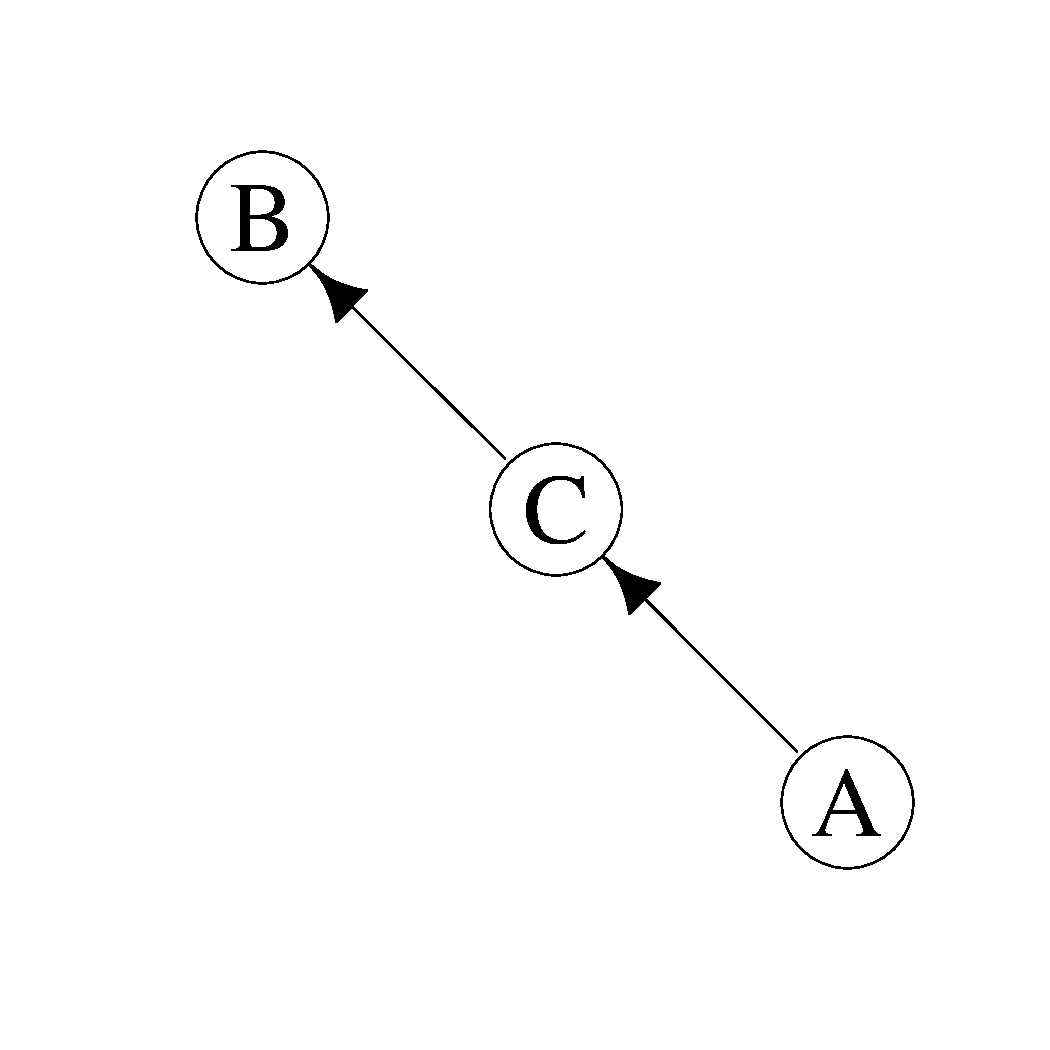
\includegraphics[width=2in]{figure/unnamed-chunk-1-1} 

\end{knitrout}

\section*{8.11}
Consider the example of the car fuel system shown in Figure 8.21, and suppose
that instead of observing the state of the fuel gauge G directly, the gauge is seen by
the driver D who reports to us the reading on the gauge. This report is either that the
gauge shows full D = 1 or that it shows empty D = 0. Our driver is a bit unreliable,
as expressed through the following probabilities
$$p(D = 1|G = 1) = 0.9$$
$$p(D = 0|G = 0) = 0.9.$$
Suppose that the driver tells us that the fuel gauge shows empty, in other words
that we observe D = 0. Evaluate the probability that the tank is empty given only
this observation. Similarly, evaluate the corresponding probability given also the
observation that the battery is flat, and note that this second probability is lower.
Discuss the intuition behind this result, and relate the result to Figure 8.54.

\begin{solution}
We can conceive of the problem in terms of a graph like this, wherein we've observed $D$:

\begin{knitrout}
\definecolor{shadecolor}{rgb}{0.969, 0.969, 0.969}\color{fgcolor}\begin{kframe}
\begin{alltt}
\hlstd{g} \hlkwb{<-} \hlkwd{graph_from_literal}\hlstd{(F}\hlopt{-+}\hlstd{G}\hlopt{+-}\hlstd{B, G}\hlopt{-+}\hlstd{D)}
\hlkwd{plot.igraph}\hlstd{(g,} \hlkwc{edge.color} \hlstd{=} \hlstr{"black"}\hlstd{,} \hlkwc{vertex.color} \hlstd{=} \hlstr{"white"}\hlstd{,}
            \hlkwc{vertex.label} \hlstd{=} \hlkwd{c}\hlstd{(}\hlstr{"F"}\hlstd{,}\hlstr{"G"}\hlstd{,}\hlstr{"B"}\hlstd{,} \hlstr{"D"}\hlstd{),} \hlkwc{vertex.size} \hlstd{=} \hlnum{45}\hlstd{,} \hlkwc{vertex.label.cex} \hlstd{=} \hlnum{4}\hlstd{,}
            \hlkwc{vertex.label.color} \hlstd{=} \hlstr{"black"}\hlstd{,} \hlkwc{edge.width} \hlstd{=} \hlnum{1}\hlstd{,} \hlkwc{edge.arrow.size} \hlstd{=} \hlnum{2}\hlstd{,}
            \hlkwc{edge.arrow.width} \hlstd{=} \hlnum{1.2}\hlstd{)}
\end{alltt}
\end{kframe}
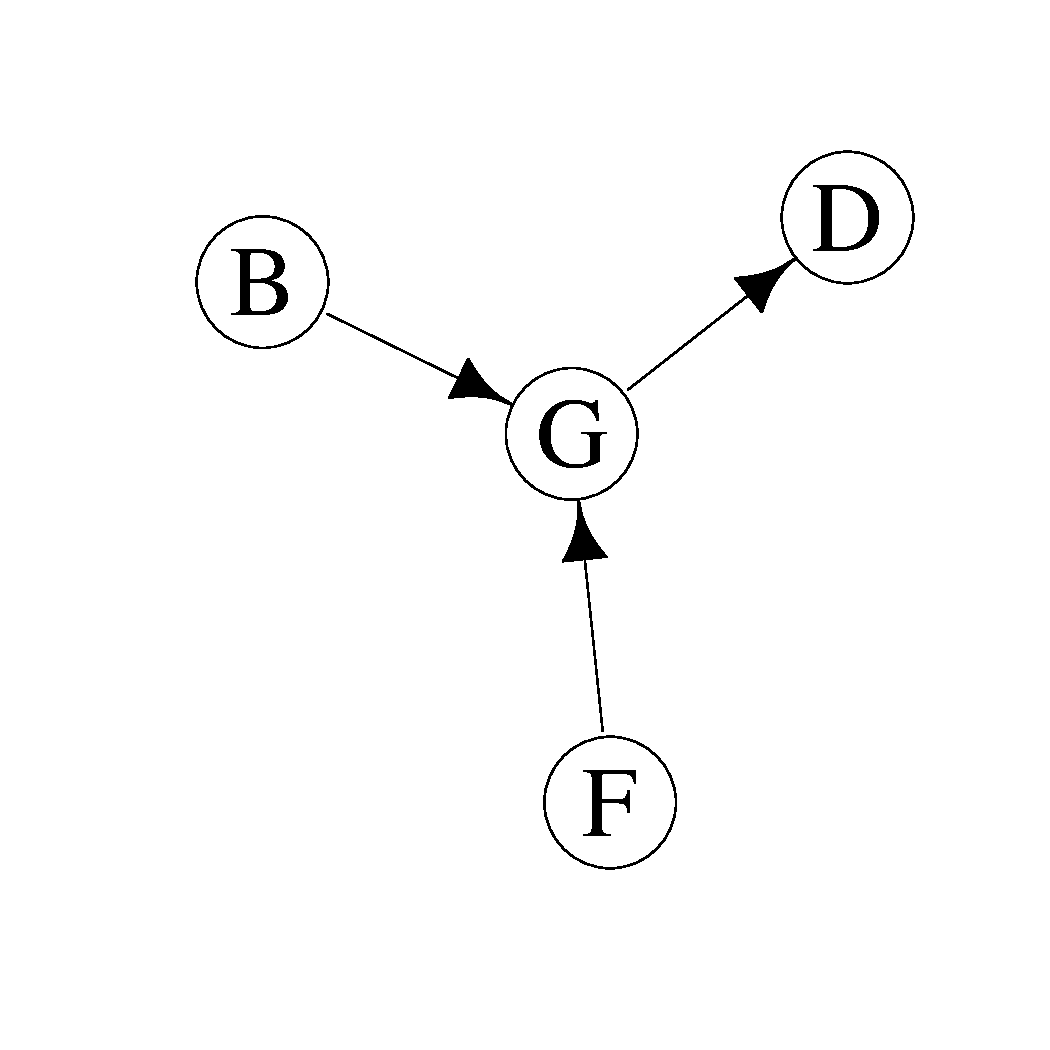
\includegraphics[width=2in]{figure/unnamed-chunk-2-1} 

\end{knitrout}

We have the following prior probabilities regarding whether the battery is charged or flat and whether the tank is full or empty:

$$P(B=1) = 0.9$$
$$P(F=1) = 0.9.$$

And we know that, given the state of the fuel tank and the battery, the fuel gauge reads full with probabilities given by

$$p(G = 1|B = 1, F = 1) = 0.8$$
$$p(G = 1|B = 1, F = 0) = 0.2$$
$$p(G = 1|B = 0, F = 1) = 0.2$$
$$p(G = 1|B = 0, F = 0) = 0.1$$

We know that we have a prior $p(F=0) = 0.1$. Following the graph, we can find the evidence term -- the denominator for the posterior -- like this

\begin{align}
p(D=0) &= \sum_G \sum_F \sum_B p(D=0|G)p(G|F, B)p(F)p(B) \\
&= 0.352
\end{align}

and the likelihood $p(D=0|F=0)$

\begin{align}
&= \sum_G \sum_B p(D=0|G)p(G|B,F=0)p(B) \\
&= 0.748.
\end{align}

Thus, we can compute the posterior probability that the tank is empty
\begin{align}
p(F=0|D=0) &= \frac{0.1\times0.748}{0.352} \\
&= 0.2125
\end{align}

If we receive new information, and it turns out that the battery is definitely flat, we can recompute the posterior for the status of the fuel gauge. We can use the same prior $p(B=0) = 0.1$. But now, we rearticulate the evidence and likelihood accordingly: \newline

New evidence:
\begin{align}
p(D=0|B=0) &= \sum_G \sum_F p(D=0|G)p(G|F, B=0)p(F) \\
&= 0.81
\end{align}

New likelihood:
\begin{align}
p(D=0|B=0, F=0, G) &= \sum_G p(D=0|G)(G|B=0, F=0)\\
&= 0.82
\end{align}

And thus, the new posterior:
\begin{align}
p(F=0|D=0, B=0) &= \frac{0.1\times0.82}{0.81}\\
&\approx 0.101
\end{align}

We see that the posterior probability given the information about the battery's status -- specifically, that it is flat -- is less than the posterior probability before we had this information. Intuitively, this is because the battery's being flat is likely to account, at least partly, for the gauge reading 0 -- and thus, for the driver reporting 0 on the gauge. 

\end{solution}

\end{document}
